% *********************************************************************
% © 2021-2023 Jeremy Sylvestre
%
% Permission is granted to copy, distribute and/or modify this document
% under the terms of the GNU Free Documentation License, Version 1.3 or
% any later version published by the Free Software Foundation; with no
% Invariant Sections, no Front-Cover Texts, and no Back-Cover Texts. A
% copy of the license is included in the appendix entitled “GNU Free
% Documentation License” that appears in the output document of this
% PreTeXt source code. All trademarks™ are the registered® marks of
% their respective owners.
%
% *********************************************************************

\newcommand*{\xmin}{-8}
\newcommand*{\xmax}{17}
\newcommand*{\ymin}{-1}
\newcommand*{\ymax}{2.75}

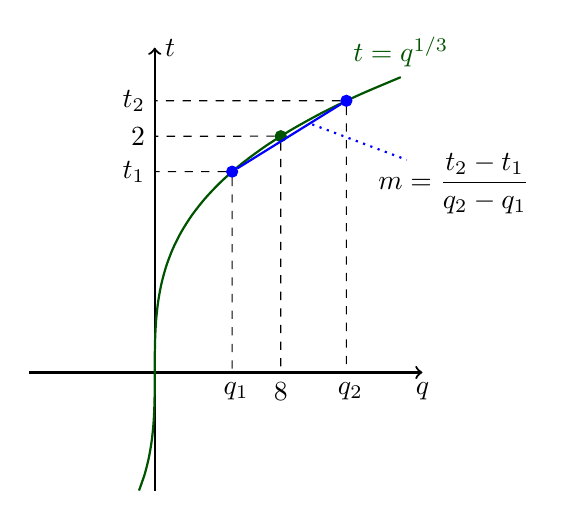
\begin{tikzpicture}
[
	closedpt/.style={circle,draw,fill,inner sep=0pt,minimum size=4pt},
	openpt/.style={circle,draw,inner sep=0pt,minimum size=4pt},
	xscale=0.2,yscale=1.5
]

	% axes
	\draw[->,thick] (\xmin,0) -- (\xmax,0) node[below] {$q$};
	\draw[->,thick] (0,\ymin) -- (0,\ymax) node[right] {$t$};

	\draw[green!33!black,thick,domain=-1:2.5,smooth] plot ({\x * \x * \x},\x) node[above] {$t = q^{1/3}$};

	\node[closedpt,green!33!black] at (8,2) (pt) {};
	\node[closedpt,blue] at (4.913,1.7) (pt1) {};
	\node[closedpt,blue] at (12.167,2.3) (pt2) {};

	\draw[dashed] (pt) -- (0,2) node[left] {$2$};
	\draw[dashed] (pt) -- (8,0) node[below] {$8$};

	\draw[dashed] (pt1) -- (0,1.7) node[left] {$t_1$};
	\draw[dashed] (pt1) -- (4.913,0) node[below,xshift=0.05cm] {$q_1$};
	\draw[dashed] (pt2) -- (0,2.3) node[left] {$t_2$};
	\draw[dashed] (pt2) -- (12.167,0) node[below,xshift=0.05cm] {$q_2$};
	\draw[blue,thick] (pt1) -- (pt2);

	\draw[dotted,blue,thick] (10,2.1) -- (16,1.8);
	\node at (19,1.6) {$\displaystyle m = \frac{t_2 - t_1}{q_2 - q_1}$};

\end{tikzpicture}
